\documentclass[11pt, oneside]{article} 
\usepackage{geometry}
\geometry{letterpaper} 
\usepackage{graphicx}
	
\usepackage{amssymb}
\usepackage{amsmath}
\usepackage{parskip}
\usepackage{color}
\usepackage{hyperref}

\graphicspath{{/Users/telliott_admin/Dropbox/Tex/png/}}
% \begin{center} 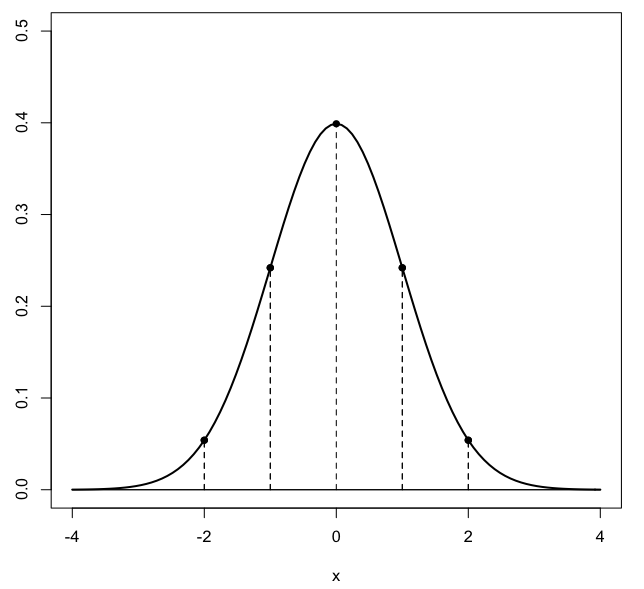
\includegraphics [scale=0.4] {gauss3.png} \end{center}

\title{Geometric rotation}
\date{}

\begin{document}
\maketitle
\Large


\label{sec:Geometric_rotation}

Our goal here is to find the equations for rotation of coordinates.  We want to be as simple as we can, so that we can (at least try to) remember how the derivation works.

In this chapter we look at geometric approaches.  Vector methods are simpler, in my opinion, but they require knowing the idea of matrix multiplication.  The geometry can be confusing to set up, but once that's done you can just read the answer off the diagram.

\subsection*{Stewart}
I found a nice method in Stewart that depends on knowing the sum of angles formulas, which I urged you to memorize.
\begin{center} 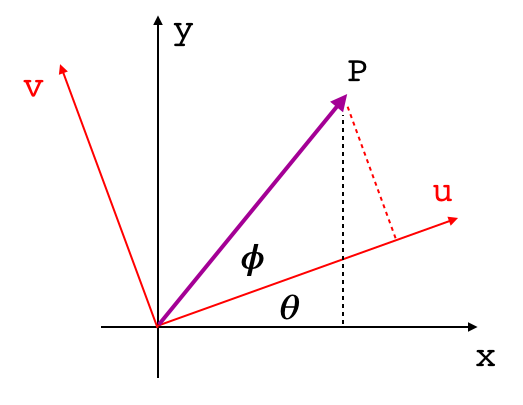
\includegraphics [scale=0.4] {min_rotation3.png} \end{center}

Here, we have the standard $xy$-coordinates in black.  The rotated $uv$-coordinate system is in red, with a rotation angle $\theta$ in the counter-clockwise direction.

The ray to the point $P$ has length $r$.  Notice that the coordinates of point $P$ in the $u,v$ system are naturally expressed in terms of $\phi$:
\[ u = r \cos \phi \]
\[  v = r \sin \phi \]
while $x$ and $y$ are naturally expressed in terms of the combined angle $\theta + \phi$.
\[ x = r \cos (\theta + \phi) \]
Now, use the sum formula for cosine: 
\[ x = r \cos \theta \cos \phi - r \sin \theta \sin \phi \]
But we have from above that
\[ u = r \cos \phi \]
\[ v = r \sin \phi \]
So
\[ x = u \cos \theta - v \sin \theta \]
It's as easy as that.

In the same way:
\[ y = r \sin (\theta + \phi) \]
\[ = r \sin \theta \cos \phi + r \cos \theta \sin \phi \]
\[ = u \sin \theta + v \cos \theta \]

\subsection*{Solve for u and v}
To convert these formulas to functions $u = f(x,y)$ and $v = f(x,y)$, there is a hard way and an easy way.  We do the hard way first:
\[ x = u \cos \theta - v \sin \theta \]
so
\[ x \cos \theta = u \cos^2 \theta - v \sin \theta \cos \theta \]
and
\[ y = u \sin \theta + v \cos \theta \]
so
\[ y \sin \theta = u \sin^2 \theta + v \sin \theta \cos \theta \]
adding:
\[ x \cos \theta + y \sin \theta = u \]
similarly:
\[ x \sin \theta = u \sin \theta \cos \theta - v \sin^2 \theta \]
\[ y \cos \theta = u \sin \theta \cos \theta + v \cos^2 \theta \]
add minus the first to the second:
\[ - x \sin \theta + y \cos \theta = v \]
    
It \emph{is} easier when you know where you're going.  In summary:
\[ u =  x \cos \theta + y \sin \theta \]
\[ v = - x \sin \theta + y \cos \theta \]
and the original pair:
\[ x = u \cos \theta - v \sin \theta \]
\[ y = u \sin \theta + v \cos \theta \]
The difference is the sign of the sine.

The easy way is to switch $x,y$ for $u,v$ and at the same time, substitute $-\theta$ for $\theta$.  What this amounts to is relabeling our diagram with $x,y$ being the rotated axes, and then rotating in the opposite direction (cw rather than ccw).
\[ x = u \cos \theta - v \sin \theta \]
switch
\[ u = x \cos -\theta - y \sin -\theta \]
\[ = x \cos \theta + y \sin \theta \]
(Recall that $\cos - x = \cos x$ and $\sin - x = - \sin x$).

For $y$
\[ y = u \sin \theta + v \cos \theta \]
switch
\[ v = x \sin -\theta + y \cos -\theta \]
\[ v = -x \sin \theta + y \cos \theta \]

\subsection*{A small test}

Rotation of coordinates counter-clockwise ($x,y$ to $u,v$) gives $- \sin$ in the formula for the vertical component $v$), whereas clockwise rotation ($u,v$ to $x,y$) gives $- \sin$ in the formula for the horizontal component $x$.

One way to see that this is correct is to substitute from the $u,v$ formulas into the $x,y$ ones:
\[ x = (x \cos \theta + y \sin \theta) \cos \theta - (- x \sin \theta + y \cos \theta) \sin \theta \]
    
Can you see that if this is multiplied out, we will get $x (\cos^2 \theta + \sin^2 \theta) = x$ and the terms with $y$ will just cancel?

A similar thing happens with the other one:
\[ y = (x \cos \theta + y \sin \theta) \sin \theta + (- x \sin \theta + y \cos \theta) \cos \theta = y \]

\subsection*{standard derivation}
Here is a second derivation with a sort of minimalist diagram of rotation
\begin{center} 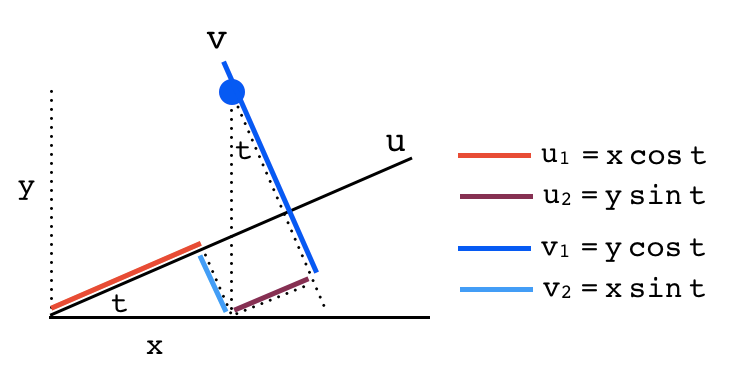
\includegraphics [scale=0.5] {min_rotation.png} \end{center}

We draw the horizontal $x$-axis and the rotated $u$-axis.  The angle between them is $t$.  We plot our point and then draw perpendiculars to both axes.  To finish the set-up, we draw perpendiculars from the point $(x,0)$ as shown.

Once the drawing is rendered, we are almost done.  You will know that you've done it right if you have both $x$ and $y$ as the \emph{hypotenuse of a right triangle}.  Now we just work our way through

\[ u_1 = x \cos t \]
\[ u_2 = y \sin t \]
So 
\[ u = x \cos t + y \sin t \]

(All the triangles in the diagram are similar, with small angle $t$.  Can you prove it?)
\[ v_1 = y \cos t \]
\[ v_2 = x \sin t \]
\[ v = -  x \sin t + y \cos t \]

\subsection*{Shankar derivation}
It seems that the more you talk about rotation, the less clear things become.  Nevertheless, I will show one more from Shankar's book, and then work through a calculation.
\begin{center} 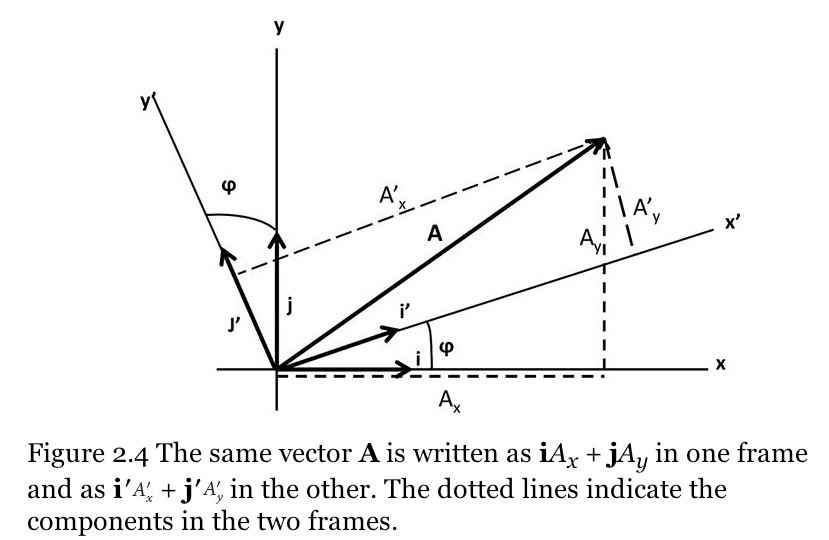
\includegraphics [scale=0.4] {Shankar_rotation.png} \end{center}

Write $\mathbf{\hat{i}}'$ in terms of $\mathbf{\hat{i}}$ and $\mathbf{\hat{j}}$ as follows.  

To reach the end of $\mathbf{\hat{i}}'$ we go out in the $\mathbf{\hat{i}}$ direction.  How far?  Call it $x$.  In terms of the new unit vector $\mathbf{\hat{i}}'$ we have
\[ \frac{x}{|\mathbf{\hat{i}}'|} = \cos \phi \]
But $|\mathbf{\hat{i}}'| = 1$ so
\[ x = \cos \phi \]
$x$ is shorter than $\mathbf{\hat{i}}$ by the factor of $\cos \phi$.

We also need to go up in the $\mathbf{\hat{j}}$ direction.  Use the other triangle with $\mathbf{\hat{j}}$ rotated to $\mathbf{\hat{j}}'$ (which is similar to the first triangle).

\[ \frac{y}{|\mathbf{\hat{j}}'|} = \sin \phi \]
But $|\mathbf{\hat{j}}'| = 1$ so
\[ y = \sin \phi \]
$y$ is shorter than $\mathbf{\hat{j}}$ by the factor of $\sin \phi$.

\begin{center} 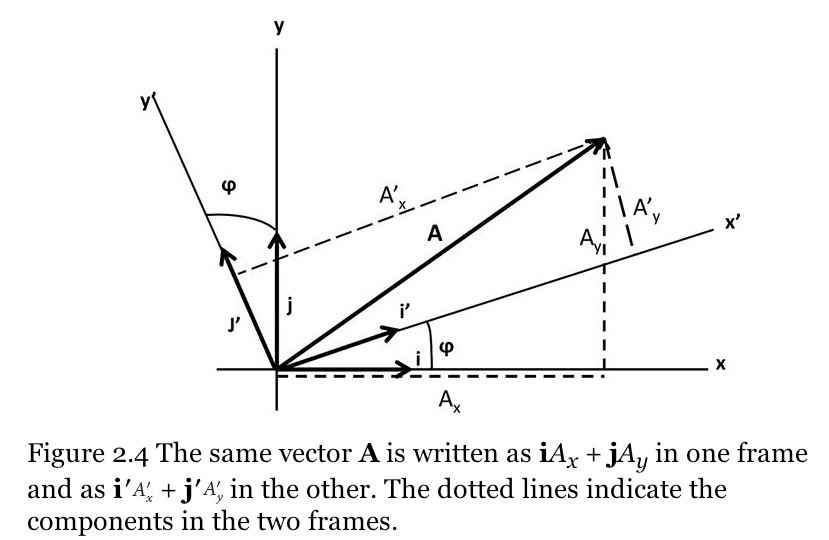
\includegraphics [scale=0.4] {Shankar_rotation.png} \end{center}
So to construct $\mathbf{\hat{i}}'$ we go out in the $\mathbf{\hat{i}}$ direction a distance of $\cos \phi$ and up in the $\mathbf{\hat{j}}$ direction a distance of $\sin \phi$:

\[ \mathbf{\hat{i}}' = \mathbf{\hat{i}} \cos \phi + \mathbf{\hat{j}} \sin \phi \]
A similar process will yield
\[ \mathbf{\hat{j}}' = \mathbf{\hat{j}} \cos \phi - \mathbf{\hat{i}} \sin \phi \]

Now write the vector $\mathbf{A}$ in two ways:
\[ \mathbf{A} = A_x' \ \mathbf{\hat{i}}' + A_y' \ \mathbf{\hat{j}}'  \]
\[ = (\mathbf{\hat{i}} \cos \phi + \mathbf{\hat{j}} \sin \phi) A_x' + (\mathbf{\hat{j}} \cos \phi - \mathbf{\hat{i}} \sin \phi) A_y' \]
\[ = \mathbf{\hat{i}}(\cos \phi A_x' - \sin \phi A_y') + \mathbf{\hat{j}}(\sin \phi A_x' + \cos \phi A_y') \]
or in the usual way
\[ \mathbf{A} = A_x \ \mathbf{\hat{i}} + A_y \ \mathbf{\hat{j}}  \]

So
\[ A_x = \cos \phi \ A_x' - \sin \phi \ A_y' \]
\[ A_y = \sin \phi \ A_x' + \cos \phi \ A_y' \]

Finally compute the length of $\mathbf{A}$ (squared):
\[ A_x^2 =   \cos^2 \phi \ {A_x'}^2 + \sin^2 \phi \ {A_y'}^2 - 2 \cos \phi \ {A_x'}\ \sin \phi \ A_y' \]
\[ A_y^2 = \sin^2 \phi \ {A_x'}^2 + \cos^2 \phi \ {A_y'}^2 + 2 \sin \phi \ {A_x'} \  \cos \phi \ {A_y'} \]
Add together and notice the cancellation of the mixed $A_x'$ and $A_y'$ terms:
\[ A_x^2 + A_y^2 = \cos^2 \phi \ {A_x'}^2 + \sin^2 \phi \ {A_y'}^2 + \sin^2 \phi \ {A_x'}^2 + \cos^2 \phi \ {A_y'}^2 \]
\[ = {A_x'}^2 + \sin^2 \phi \ {A_y'}^2 + \cos^2 \phi \ {A_y'}^2 \]
\[ = {A_x'}^2 + {A_y'}^2 \]
As we should expect, the length of a vector such as $\mathbf{A}$ is \emph{invariant}, it does not depend on the choice of coordinate system.

\end{document}